\section{Zweierkomplement}

\begin{frame}{Ein asymetrischer Zahlenbereich}
	\[
	\nK_{\ell} = \{ x\in \Z\mid -2^{\ell-1} \leq x \leq 2^{\ell-1} -1 \} \;.
	\]
	\\[0.2cm]
	
	\begin{figure}
		\centering
		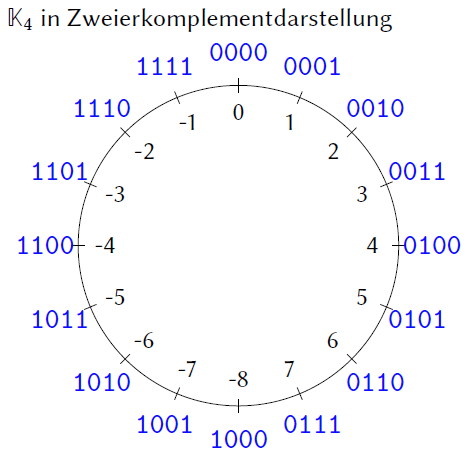
\includegraphics[scale=0.45]{ZK_K4}
	\end{figure}
	
\end{frame}

\begin{frame}{Zweierkomplement}

	Das Zweierkomplement ist eine Möglichkeit, negative Zahlen binär darzustellen. Im Vergleich zu anderen Darstellungsarten ist es besonders vorteilhaft bei arithmetischen Rechnungen mit Hardware \textit{(mehr dazu in Technischer Informatik)}.

	\begin{block}{Definition}
		$$Zkpl_l(x) = \begin{cases} 0 bin_{l-1}(x) & \text{falls } x \geq 0 \\ 1 bin_{l-1}(2^{l-1}+x) & \text{falls } x < 0\end{cases}$$
		
		Äquivalent:
		$$Zkpl_l(x) = \begin{cases} bin_{l}(x) & \text{falls } x \geq 0 \\ bin_{l}(2^{l}+x) & \text{falls } x < 0\end{cases}$$
	\end{block}
\end{frame}

\begin{frame}{ZK-Beispiel}
	\begin{block}{Beispiele}
		\begin{align*}
			&Zkpl_5(0) \only<2->{= 00000} \\
			&Zkpl_5(2) \only<3->{= 00010} \\
			&Zkpl_5(15) \only<4->{= 01111} \\
			&Zkpl_5(-1) \only<5->{= 11111} \\
			&Zkpl_5(-6) \only<6->{= 11010} \\
			&Zkpl_5(-16) \only<7->{= 10000}
		\end{align*}
	\end{block}
\end{frame}

\begin{frame}{ZK: Einfache Berechnung}
	Zum \enquote{intuitiven} Berechnen des Zweierkomplement können wir so vorgehen (für $x < 0$):
	\begin{enumerate}
		\item Binärdarstellung von $\setsize{x}$ berechnen
		\item Mit führenden Nullen auffüllen bis zur Länge $\ell$
		\item Alle binären Ziffern negieren
		\item 1 addieren
	\end{enumerate}

	\begin{Beispiel}
		$$Zkpl_4(-2): 2 \rightarrow 10 \rightarrow 0010 \rightarrow 1101 \rightarrow 1110 $$
	\end{Beispiel}
\end{frame}

\begin{frame}{ZK: Einfache Berechnung}
	Die einzelnen Schritte können wir auch formal angeben:\\
	(Wir operieren jeweils auf Wörtern aus $\{0, 1\}^* = Z_2^*$) \\[0.5em]
	1. Binärdarstellung von $\setsize{x}$ berechnen: $Repr_2(\setsize{\cdot})$ \\
	2. Mit führenden Nullen auffüllen bis zur Länge $\ell$\\ \pause
	\begin{align*}
		Fill_\ell : Z_2^m &\to Z_2^\ell \qquad (m \le \ell) \\ \visible<3-> {
		w &\mapsto \begin{cases}
		0^\ell & w = \varepsilon \\
		Fill_{\ell-1}(w') \cdot \mu & w = w' \cdot \mu, w' \in Z_2^*, \mu \in Z_2
		\end{cases} \\
		&\text{oder deutlich einfacher} \\
		w &\mapsto \begin{cases}
		w & \setsize{w} = \ell \\
		Fill_\ell(0w) & \text{sonst}
		\end{cases} \\
	}
	\end{align*}
	\pause[4] 3. / 4. Analog %TODO
\end{frame}